\section{Results and Analysis}
\label{sec:results}

In this section, we present the classification results from different machine learning models with different features extracted from our dataset EJShibaVoice. Then we compare Shapley values on the GeMAPs feature to find the prominent factors.

\subsection{Classification Results}
\label{sec:main}
\begin{table}[H]
	\scriptsize
	\centering
	\begin{tabular}{l|l|lllll}
		\toprule
		\multicolumn{2}{c|}{}            & xgboost & KNN  & LR   & RF  \\
		\midrule
		\multicolumn{2}{c|}{filterbank}          & 0.9827        & 0.9057         & 0.6374    & 0.9603    \\
		\multicolumn{2}{c|}{ComParE} & {0.9868} & {0.5717} & {0.6004} & {0.9520}\\
		\multicolumn{2}{c|}{GeMAPs} & 0.9836 & 0.7317 & 0.6230 & 0.9474 \\
		\multicolumn{2}{c|}{eGeMAPs} & 0.9840 & 0.7432 & 0.6901 & 0.9567\\
		\multicolumn{2}{c|}{PLP} & 0.9733 & 0.7701 & 0.4375 & 0.9123\\
		\multicolumn{2}{c|}{MFCC} & 0.9828 & 0.9161 & 0.5441 & 0.9587\\
		\bottomrule
	\end{tabular}
	\caption{Classification results on EJShibaVoice dataset. Note that the barking excerpts are under pairing scenarios, excluding other confounding factors.} %The results of main experiment which tries to correctly classify bark pairs into their host language patterns. We have tested four common models on six kinds of audio features of our EJShibaVoice dataset.}
	\label{table:mainresult}
\end{table}

The classification results are presented in \tabref{table:mainresult}, where six different audio features are compared under four classification models. Among these features, filterbank, PLP and MFCC are extracted from the spectral transformation, and have 24, 13, 13 dimensions respectively. While ComParE, GeMAPs and eGeMAPs are statistical features by human design and have 6373, 62, 88 dimensions respectively. These three features are easier to explain from acoustic angle, however, some information may get lost in the statistical transformation to cause decline in accuracy.

Among these results, the accuracy of ComParE significantly drops while using KNN, which is due to the curse of dimensionality of this 6,373 dimension feature.

Results indicate that xgboost exhibited the highest classification accuracy, with all six features revealing an accuracy higher than 0.90. No matter which feature set or model is used, high distinctiveness of dog barking from different host language environments is observed. In other words, this indicates that there is certain acoustic difference between the dog barks in these two language environments. 




\subsection{Results of Prominent Factors}
\label{sec:prominentfactor}
The results of SHAP values can be seen in \figref{fig:prominentfig} and details of the selected dimensions are listed in \tabref{table:prominentfactor}.

\begin{figure}[th]
	\centering
	\scalebox{0.5}{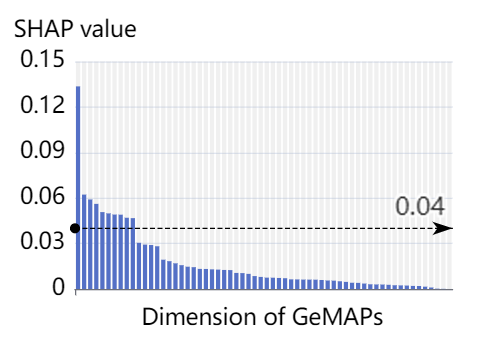
\includegraphics{images/prominent_result.png}}
	\caption{The average SHAP values (absolute value) of GeMAPs sorting from high to low. Features with SHAP values higher than 0.04 are considered prominent and will be described below.} %These values are all absolute values to make them comparable.} %\KZ{Who said 0.06 is the threshold? Cite?}%our own definition 
	\label{fig:prominentfig} %\MYW{what do you mean sorted? ranking from high to low?}
\end{figure}



\begin{table}[th]
	\scriptsize
	\centering
	\begin{tabular}{l|c|c}
		\toprule
		Dimension &SHAP  & p-value\\
		\midrule
		\textbf{loudness\_sma3\_amean} & 0.1336 & {1.0e-75}    \\
		\textbf{F0semitoneFrom27.5Hz\_sma3nz\_percentile50.0} &  0.0622  & {3.8e-4}\\
		\textbf{loudness\_sma3\_meanRisingSlope} &  0.0590  & {2.2e-6}\\
		logRelF0-H1-A3\_sma3nz\_stddevNorm  & 0.0561  & {0.92}\\
		\textbf{loudnessPeaksPerSec} & 0.0507  & {1.8e-4}\\
		\textbf{F0semitoneFrom27.5Hz\_sma3nz\_percentile80.0}  & 0.0498  & {2.9e-9}\\
		hammarbergIndexV\_sma3nz\_stddevNorm & 0.0491  & {0.71}\\
		\textbf{slopeV0-500\_sma3nz\_amean}  & 0.0490 & {2.7e-92}\\
		\textbf{loudness\_sma3\_percentile80.0} & 0.0470  & {1.6e-47}\\
		\textbf{slopeV500-1500\_sma3nz\_stddevNorm}  & 0.0467 & {5.5e-5}\\
		\bottomrule
	\end{tabular}
	\caption{Details of Prominent Dimensions. SHAP columns refer to the average SHAP values. We have analyzed the pearson value between 982 barks and speech clips. Features in bold style have p-value lower than 0.05. This indicated they have strong correlation.}
	\label{table:prominentfactor}
\end{table}

%10	0.3674 2.3e-4
%3	0.0628 0.54
%16	0.0927 0.36
%29	-0.0506 0.62
%56	-0.0278 0.79
%4	0.0019 0.98
%47	-0.0620 0.55
%48	0.6177 2.0e-11
%14	0.2817 5.4e-3
%51	-0.0090 0.93
The ten prominent factors above are grouped into four categories: spectral, temporal, energy, and frequency according to the original GeMAPS definition. Most of the prominent factors fall into Spectral parameters, including dimensions about HammerbergIndex and slope. Respectfully HammerbergIndex represents the ratio of the strongest peak in the 0-2kHz region to the strongest peak in the 2-5kHz region; Slope represents the linear regression slope of the spectral power spectrum within the given band.

F0semitone-related factors describe the pitch, which is highly related to fundamental frequency. The factors about segment length are in the category of temporal parameters. The energy-related parameter loudness, which represents the estimation of sound intensity, is usually largely influenced by the recording device and environment. Here we take it as the audio sampling difference during recording.

Considering these factors, the results show that dog barks from two host language environments have distinctive differences in their energy distribution over frequency. The segment length plays an important role as well. In quantitative analysis, barks from the Japanese language environment reveal to be higher than those from English in frequency and contain shorter length.

In order to better compare the barks with human language, we conduct a SHAP analysis on human language: open public language corpus CommonVoice and the hosts' speech extracted from the same videos as we extracted dog barking. 
%\MYW{cite refs for commonvoice. Introduce this comparison in your\part{title} method section as well.}
To find the difference between these two languages, we use xgboost as well to classify human speech and then compute Shapley values, with results presented in \figref{fig:humanspeech}.

% \MYW{This paragraph is hard to follow. You preprocessed the CommonVoice data?}
%The result can be seen at \figref{fig:humanspeech}.

\begin{figure}[th]
	\centering
	\scalebox{0.32}{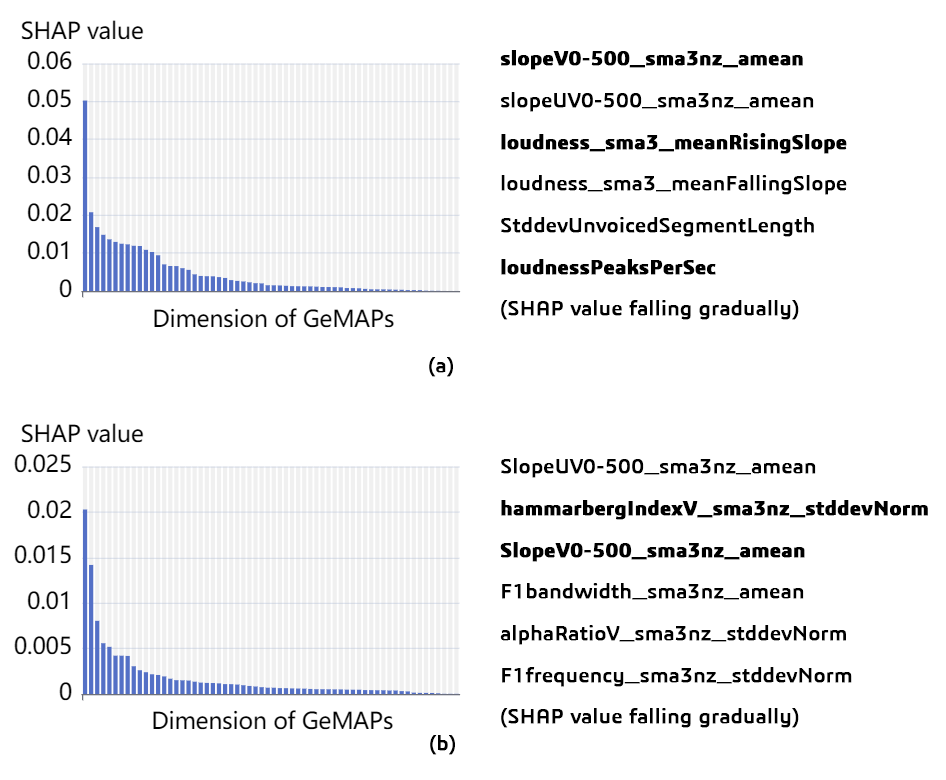
\includegraphics{images/prominent_speech.png}}
	\caption{(a) and (b) are respectfully results of SHAP analysis on open corpus and extracted human speech audios. The first six dimensions are labelled at right, and those who are overlapped with prominent factors in barks of dogs are bold.}
	\label{fig:humanspeech}
\end{figure}

% \KZ{Once we have found the common important factors between dog barks and human speeches, can we show a diagram to illustrate the correlation between dogs and human in the two communities respectively?} okok wait for me ;;;  the space is not enough now


In the human speech analysis, the difference between English and Japanese concentrates on the slope, loudness, and F0semitone. From the above, we can conclude that the difference between barks coming from different host language environments is mainly related to frequency. In the meantime, from our analysis of prominent acoustic factors, the barks of dogs and voices of humans share several same prominent factors, suggesting that the host human language have correlation with the barks of dogs.

Furthermore, to ascertain the correlation between barks and speech more directly besides the overlap of their prominent factors, we calculate the Pearson correlation between barks and speech extracted from the same videos in the ten prominent dimensions selected. the Pearson correlation is shown in the Pearson column in ~\tabref{table:prominentfactor}.


Here we list two typical samples from two language environments in~\figref{Fig.sample}. It is clear that barks in the English environment contain more unvoiced segments(the blue part) while the frequency of those barks in the Japanese environment is closer to the low-frequency region.

\begin{figure}[ht]
	\centering

	\subfigure[Barks under Japanese Env.]{
		\label{Fig.subja}
		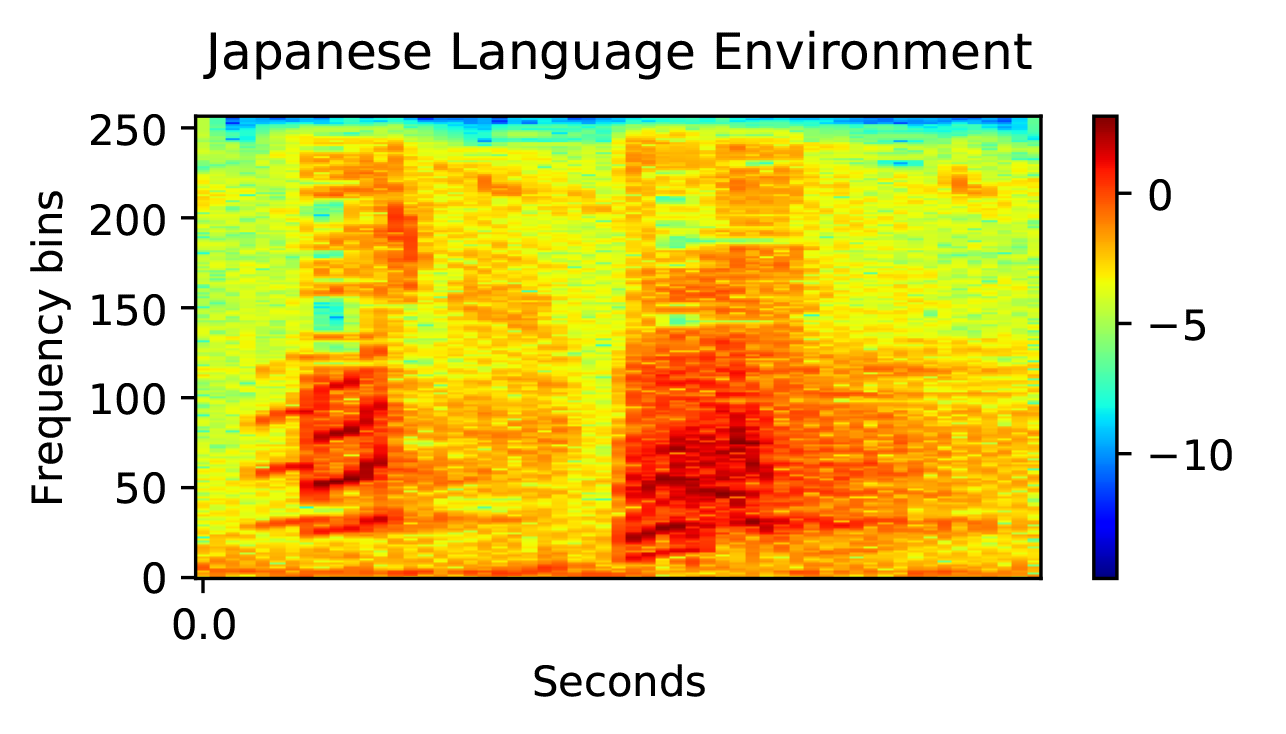
\includegraphics[width=0.48\linewidth]{dog_spec_ja_1.png}}
	\subfigure[Barks under English Env.]{
		\label{Fig.suben}
		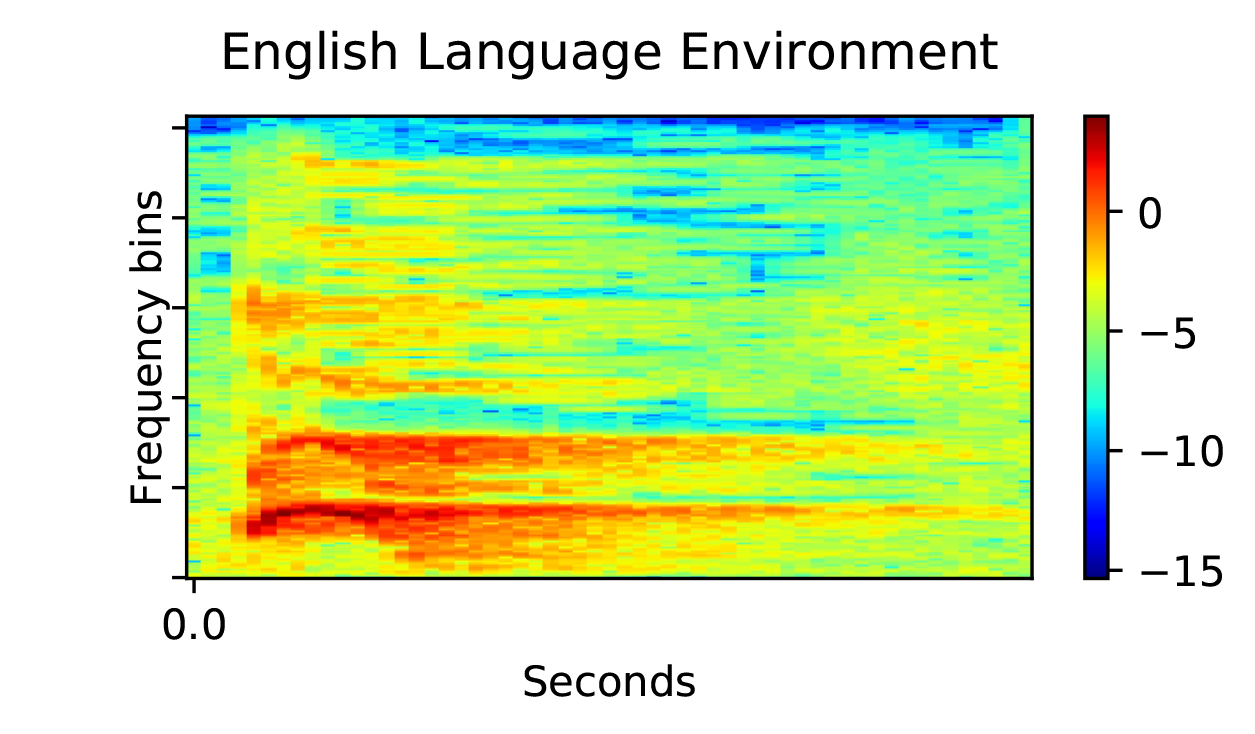
\includegraphics[width=0.48\linewidth]{dog_spec_en_1.png}}
	\caption{The spectrogram of two audio samples which are from different language environments. There are in the similar situations.}
	\label{Fig.sample}
\end{figure}


In addition, we conducted a subjective evaluation by humans to bolster our results. The evaluation contains 20 pairs of barks from different host language environments, given out to 30 participants, making up 600 items in total. Results indicated that 59.00\% participants can distinguish differences between a pair, and 79.09\% agree that the difference lies in pitch, which is the auditory perceptive expression of frequency. The results are in pair with our statistical analysis.
% In addition to the acoustic analysis, we also try to observe the difference of dog barks under different host language environment from a human perspective through questionnaires. Thus we select 20 pairs of bark clips with different language environment from \secref{sec:method}. People are required to distinguish in three points of view: urgency, pitch and duty ratio. The questionnaires include 30 pairs for 20 people each. 

%People should first judge whether there are  differences between the two clips. If the answer is yes, they need to judge the two clips from the following four dimensions: (1)urgency (2)pitch (3)duty ratio, which is the ratio of the duration of the voiced segments to the duration of the unvoiced segments (4)loudness. \\

% It should be noted that for each dimension, people can only choose which clip performs higher on this dimension or there is no obvious difference. The order inside each pair is shuffled randomly. 30 questionnaires are collected for each pair, resulting in a total of 600 questionnaires. 

% 59.00\% of the questionnaires report there are differences between the two clips of a pair, which shows that humans can tell the difference between dog barks from different host languages. Also, 79.09\% of the questionnaires which says that there are  differences between the two clips reports one of the clip performs higher on the dimension pitch, it's higher than 74.01\%, 67.23\%, 63.56\% for the other three dimensions respectively. This shows that from a human perspective the differences are most revealed by pitch, which is highly frequency related. This is in line with our acoustic analysis.

%\KZ{Maybe we can show the spectrum of human voices between jap and english as well since we have some space?}%reply: there is no room for spectrum between jap and english.
% \MYW{Adding in the human perception analysis? Indicating 1)humans can tell the difference between dog barks from different host languages 2)the prominent factors are in line with our acoustic analysis}